\newpage
\section{Introduction}
\label{sec:introduction}
% state the learning objective 

The objective of this laboratory assignment is to choose the best architecture of the circuit in order to build a Bandpass filter using OP AMP. This assignment allowed us to deal with important concepts such as OP AMP and its diverse utility in circuits. We did this while paying attention to the merit of the project designed.\\
This merit is calculated exactly as the next equation:

\begin{equation} 
M = \frac{1}{cost * (gain deviation + central frequency deviation + 1e-6)}
\label{eq1}
\end{equation}

Being the cost the following:
\begin{itemize}
	\item cost = cost of resistors  + cost of capacitors + cost of transistors
	\item cost of resistors = 1 monetary unit (MU) per kOhm
	\item cost of capacitors = 1 MU/$\mu$F
	\item cost of transistors = 0.1 MU per transistor
	
\end{itemize}

\begin{figure}[H] 
\centering
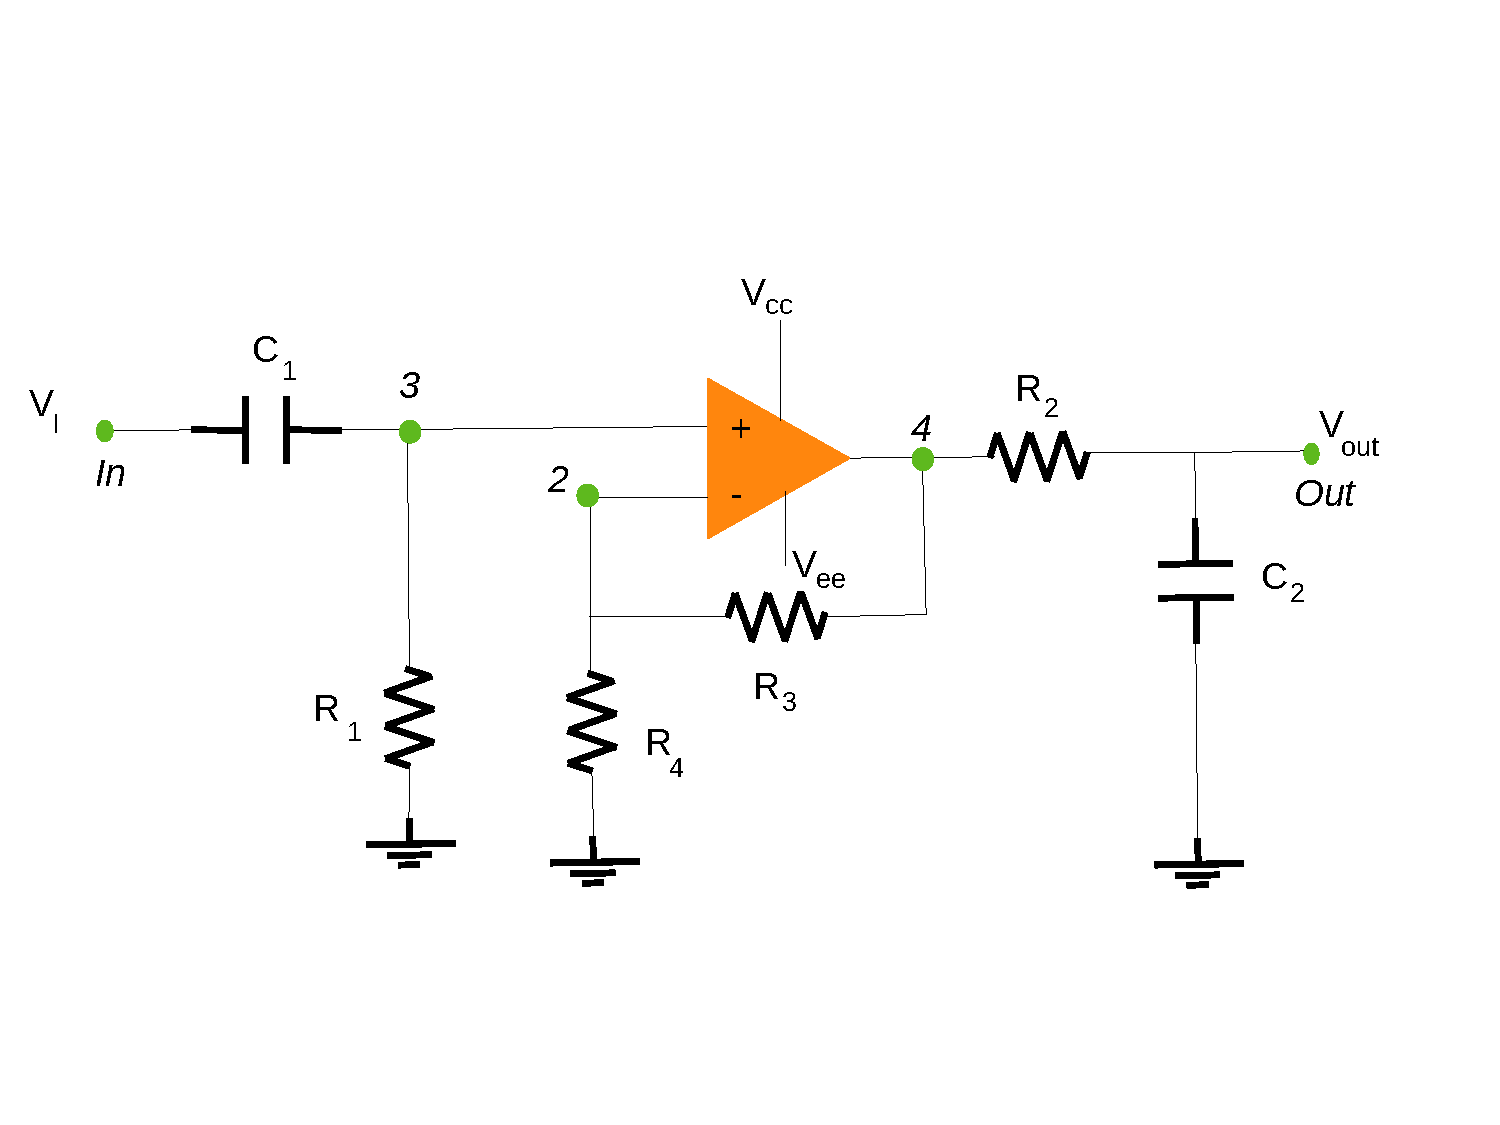
\includegraphics[width= 10cm]{circuito5.pdf} 
\caption{Main circuit}
\label{first}
\end{figure}

The constants values used are expressed in the following table.

%VALORES INTRO
\begin{table}[H] \centering
\begin{tabular}{|
>{\columncolor[HTML]{FFCC67}}l |c|}
\hline
\multicolumn{2}{|l|}{\cellcolor[HTML]{EABD8B}Name - Value} \\ \hline
C1 & 2.200000e-07 \\ \hline
C2 & 1.100000e-07 \\ \hline
R1 & 1.000000e+03 \\ \hline
R2 & 1.000000e+03 \\ \hline
R3 & 1.000000e+05 \\ \hline
R4 & 1.000000e+03 \\ \hline
Vcc & 1.000000e+01 \\ \hline

\end{tabular}
\caption{Initial Values}
\end{table}

In Section~\ref{sec:analysis}, a theoretical analysis of the circuit is
presented. In Section~\ref{sec:simulation}, the circuit is analysed by
simulation, and in Section~\ref{comparison} the results are compared to the theoretical results obtained in
Section~\ref{sec:analysis}. Next in Section~\ref{merit} we show the cost and merit atribuited to our circuit.
To finish, the conclusions of this study are outlined in Section~\ref{sec:conclusion}. \\


